%% Licensed as Creative Commons 3.0 BY SA
%% Authors: Thorsten 'Atsutane' Toepper

\documentclass[mode=print,paper=screen,size=11pt,style=simple]{powerdot}
\usepackage[utf8]{inputenc}
\usepackage{amsmath}
\usepackage{amsfonts}
\usepackage{amssymb}
\usepackage{color}
\usepackage{graphicx}
\usepackage{ngerman}
\usepackage{url}
\usepackage{listings}

\newcommand{\Anf}[1]{\glqq #1\grqq}

\lstset{
	basicstyle=\footnotesize\ttfamily,
	numbers=left,
	numberstyle=\tiny,
	xleftmargin=10pt,
	numbersep=10pt,
}

%% Symbols used in itemize sections
\def\labelitemi{\small$\blacktriangleright{}$}
\def\labelitemii{\small$\triangleright{}$}
\def\labelitemiii{\small$\bullet{}$}
\def\labelitemiv{\small\textdiamond{}}


\pddefinetemplate{titleslide}{
  titlefont=\large\bfseries\centering,
  clockpos={.99\slidewidth,\slideheight},
  lfpos={.03\slidewidth,.04\slideheight},
  rfpos={.97\slidewidth,.04\slideheight},
  texthook=t,textpos={.50\slidewidth,.7\slideheight},
  textwidth=.9\slidewidth,textfont=\centering,
  textheight=.66\slideheight
}{%
  \psline[linewidth=.8pt](0,.9\slideheight)(\slidewidth,.9\slideheight)%
  \psline[linewidth=.8pt](0,.1\slideheight)(\slidewidth,.1\slideheight)%
}
\pddefinetemplate{basic}{
  titlepos={.05\slidewidth,.93\slideheight},
  titlewidth=.9\slidewidth,textheight=.66\slideheight,
  titlefont=\large\bfseries\raggedright,
  clockpos={.99\slidewidth,\slideheight},
  lfpos={.03\slidewidth,.04\slideheight},
  rfpos={.97\slidewidth,.04\slideheight},
  tocslidesep=.6ex,textheight=.68\slideheight,
  ifsetup=portrait,
    textpos={.05\slidewidth,.83\slideheight},
    textwidth=.9\slidewidth,
    tocsecsep=.6ex,
    stochook=tr,stocpos={.48\slidewidth,.09\slideheight},
    stocfont=\tiny\raggedleft,
    ntocpos={.52\slidewidth,.09\slideheight},
  ifsetup=landscape,
    textpos={.2\slidewidth,.83\slideheight},
    textwidth=.75\slidewidth
}{%
  \psline[linewidth=.8pt](0,.9\slideheight)(\slidewidth,.9\slideheight)%
  \psline[linewidth=.8pt](0,.1\slideheight)(\slidewidth,.1\slideheight)%
  \rput(1.2,.50){\color{black}\begin{tiny}COBOL\end{tiny}}
  \rput(6,.50){\color{black}\begin{tiny}Thorsten T\"{o}pper - Proseminar Hochschule Mannheim - 9. Juni 2010\end{tiny}}
}

\author{Thorsten T\"{o}pper\\
	Proseminar Hochschule Mannheim}
\title{COBOL - COmmon Business-Oriented Language}
\pdsetup{palette=default}

\begin{document}

\maketitle
\begin{slide}{Inhalt}
  \tableofcontents[content=sections]
\end{slide}


%% Kurze Erläuterung wie und weshalb COBOL entstand
\section{Entstehung}
\begin{slide}{Entstehung}
	\begin{itemize}
		\item{Zur Entwicklung kaufmännischer Systeme entwickelt}
		\item{1959 von Grace Hopper spezifiziert}
		\item{Entwicklung wurde vom \textit{US Department of Defense} (US-Verteidigungsministerium) gesponsort}
		\item{1960 zum Standard erklärt}
	\end{itemize}
\end{slide}



%% Die weiterführende Geschichte der Sprache
\section{Geschichte}
\begin{slide}{Geschichte}
	\begin{itemize}
		\item{1968: ANS COBOL 68}
		\item{1974: COBOL 74}
		\item{1985: COBOL 85}
		\item{2002: COBOL 2002 - ISO/IEC 1989:2002}
	\end{itemize}
\end{slide}



%% Betrachtung der Vor- und Nachteile der Sprache
\section{Vor- und Nachteile}
\begin{slide}{Pro}
	\begin{itemize}
		\item{Standard}
		\item{Code für damalige Verhältnisse portabel}
		\item{Auf kaufmännische Applikationen ausgelegt}
		\item{Noch weit verbreitet $\Rightarrow$ erhöhte Jobsicherheit}
	\end{itemize}
\end{slide}


\begin{slide}{Contra}
	\begin{itemize}
		\item{Code nicht wirklich portabel}
		\item{viele zueinander inkompatible Implementierungen}
		\item{viele Dialekte}
		\item{nur globale Variablen}
		\item{Für naturwissenschaftliche Applikationen nicht geeignet}
	\end{itemize}
\end{slide}


%% Erklärung der Syntax an einem Beispielprogramm
\section{Syntax}
\begin{slide}{Syntax}
	\begin{itemize}
		\item{Syntax basiert auf Lochkarten}
	\end{itemize}
	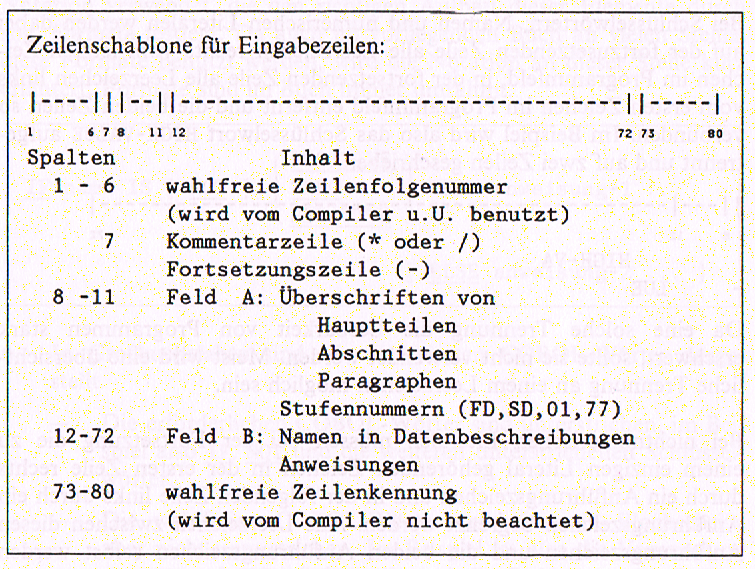
\includegraphics[scale=0.8]{syntax}\\
	Quelle: Einführung in die Programmiersprache COBOL
\end{slide}

\begin{slide}{Programmaufbau}
	\begin{itemize}
		\item{4 Hauptteile:
			\begin{itemize}
				\item{Erkennungsteil - \texttt{IDENTIFICATION DIVISION} }
				\item{Maschinenteil - \texttt{ENVIRONMENT DIVISION}}
				\item{Datenteil - \texttt{DATA DIVISION}}
				\item{Verarbeitungsteil - \texttt{PROCEDURE DIVISION}}
			\end{itemize}		
		}
	\end{itemize}
\end{slide}

\begin{slide}{Erkennungsteil}
	\begin{itemize}
		\item{Angabe von folgenden Informationen:
			\begin{itemize}
				\item{\texttt{PROGRAM-ID} - Programmname
					\begin{itemize}
						\item{Angabe an erster Stelle Pflicht}
						\item{Format des Namens divergiert bei Compilern}
					\end{itemize}				
				}
				\item{Nicht zwingend nötig:
				\begin{itemize}
					\item{\texttt{AUTHOR} - Name des Programmautors}
					\item{\texttt{INSTALLATION} - Name der Einrichtung}
					\item{\texttt{DATE-WRITTEN} - Datum der Programmerstellung}
					\item{\texttt{SECURITY} - Angabe von Sicherheitsvermerken}
				\end{itemize}
				}
			\end{itemize}		
		}
	\end{itemize}
\end{slide}

\begin{slide}{Maschinenteil}
	\begin{itemize}
		\item{Nicht zwingend notwendig}
		\item{\texttt{CONFIGURATION SECTION} - Konfigurations-Kapitel:
			\begin{itemize}
				\item{\texttt{SOURCE-COMPUTER} - Bezeichnung des Computers, auf dem kompiliert wird}
				\item{\texttt{OBJECT-COMPUTER} - Bezeichnung des Computers, auf dem ausgeführt wird}
				\item{\texttt{SPECIAL-NAMES} - verschiedene Anpassungen bspw.:
					\begin{itemize}
						\item{\texttt{DECIMAL-POINT IS COMMA.}}
					\end{itemize}				
				}
			\end{itemize}		
		}
		\item{\texttt{INPUT-OUTPUT SECTION} - Regelung der Ein- und Ausgabe:
			\begin{itemize}
				\item{\texttt{FILE-CONTROL} - Zuweisung von Geräten zu Dateien
					\begin{itemize}
						\item{\texttt{SELECT} dateiname \texttt{ASSIGN TO} systemname.}
					\end{itemize}				
				}
			\end{itemize}		
		}
	\end{itemize}
\end{slide}

\begin{slide}{Datenteil}
	\begin{itemize}
		\item{Nicht zwingend notwendig}
		\item{Unterteilt in drei Kapitel:
			\begin{itemize}
				\item{\texttt{FILE SECTION} - Deklaration interner Dateien}
				\item{\texttt{WORKING-STORAGE SECTION} - Verwaltung des Arbeitsspeichers
					\begin{itemize}
						\item{\texttt{sn var PICTURE IS datentyp VALUE IS wert.}}
					\end{itemize}				
				}
				\item{\texttt{LINKAGE SECTION} - Verbindungskapitel}
			\end{itemize}		
		}
	\end{itemize}
\end{slide}


\begin{slide}{Verarbeitungsteil}
	\begin{itemize}
		\item{Notwendig}
		\item{Enthält die Prozeduren}
	\end{itemize}
\end{slide}

\begin{slide}{Code-Beispiel: Fakultätsberechnung}
	\lstinputlisting[]{samples/faculty_1.sample}
\end{slide}

\begin{slide}{Code-Beispiel}
	\lstinputlisting[]{samples/faculty_2.sample}
\end{slide}


% Die Angabe der zur Recherche verwendeten Quellen
\section{Quellen}
\begin{slide}{Quellen}
	\begin{itemize}
		\item{\url{http://de.wikipedia.org/wiki/COBOL}}
		\item{\url{http://en.wikipedia.org/wiki/COBOL}}
		\item{\url{http://www.opencobol.org/}}
		\item{\url{http://www.cobolstandards.com/}}
		\item{Alexander Graf, Peter Sandner, Peter Stede - \\
			\textit{Einführung in die Programmiersprache COBOL}\\
			ISBN: 3-411-76481-3}
	\end{itemize}
\end{slide}


\end{document}
